\hypertarget{ux5177ux8eabux667aux80fdux7684ux6570ux636eux8303ux5f0f}{%
\chapter{具身智能的数据范式}\label{ux5177ux8eabux667aux80fdux7684ux6570ux636eux8303ux5f0f}}

\hypertarget{ux5177ux8eabux667aux80fdux8badux7ec3ux6570ux636eux6982ux8ff0}{%
\section{具身智能训练数据概述}\label{ux5177ux8eabux667aux80fdux8badux7ec3ux6570ux636eux6982ux8ff0}}

缺乏足够的训练数据是具身智能发展的一大难题。不同数据的量和价值各有不同。

\hypertarget{ux4e00ux771fux673aux6570ux636e}{%
\subsection{一、真机数据}\label{ux4e00ux771fux673aux6570ux636e}}

这是精度和价值最高的一类数据，可以由人类操作员通过遥操作设备控制真实机器人完成任务产生，也可以由经过预训练的模型自主执行任务产生（失败边缘时，人类专家可介入进行修正，产生从失误中恢复的数据）。其中，遥操作的方式较多，下面举几个例子：

\begin{enumerate}
\def\labelenumi{\arabic{enumi}.}
\item
  直接输入，人通过手柄、摇杆、键盘、鼠标、触摸屏等设备直接给机器人发送运动指令，但对高自由度任务实现难度大。
\item
  主从式，操作者控制一个``主设备''，机器人作为``从设备''同步运动，如远端机械臂跟随主机械臂的位置和姿态。
\item
  动捕，把人的动作重定向到机器人，与人的日常动作相对契合度高，但笨重的设备下人的动作容易变形、产出高质量数据效率也不够高，且部分动作机器人难以复现。
\item
  利用VR/AR设备等，操作者戴 VR 头显，在虚拟或增强现实环境中观察机器人视角，并通过手柄、手部追踪等方式控制机器人。
\end{enumerate}

优点：包含了真实世界中极其复杂的物理交互，如摩擦力、形变、复杂的接触力学以及真实的光影变化，不存在``Sim-to-Real''鸿沟。

缺点：

\begin{enumerate}
\def\labelenumi{\arabic{enumi}.}
\item
  采集成本极高，难以规模化。
\item
  依赖封闭的空间，任务和环境的多样性受限。
\end{enumerate}

\hypertarget{ux4e8cux7269ux7406ux5f15ux64ceux5408ux6210ux6570ux636e}{%
\subsection{二、物理引擎合成数据}\label{ux4e8cux7269ux7406ux5f15ux64ceux5408ux6210ux6570ux636e}}

可利用物理仿真引擎在虚拟世界中构建环境，通过强化学习或大规模并发采样获取数据。

优点：

\begin{enumerate}
\def\labelenumi{\arabic{enumi}.}
\item
  可以快速收集海量试错数据、轻易获取环境的真实状态（如物体的精确位姿、接触力）。
\item
  环境比真机数据更加多样。
\end{enumerate}

缺点：存在Sim-to-Real Gap，物理引擎无法完美模拟现实世界，特别是对于流体、柔性物体、复杂的滑动摩擦、触觉传感器，以及各种意外情况的模拟等。

\hypertarget{ux4e09ux4e92ux8054ux7f51ux89c6ux9891ux6570ux636e}{%
\subsection{三、互联网视频数据}\label{ux4e09ux4e92ux8054ux7f51ux89c6ux9891ux6570ux636e}}

互联网中存在海量的视频数据，其中蕴含了丰富的常识、物理规律以及``如何与世界交互''的知识，可用于具身模型的预训练等，帮助模型理解物理世界的基本规律。

优点：数据量大，多样性高，可增强模型跨场景的泛化能力。

缺点：

\begin{enumerate}
\def\labelenumi{\arabic{enumi}.}
\item
  人类的身体构造（自由度、肌肉骨骼系统）与机器人完全不同，存在Embodiment Gap。一段人类灵活切菜的视频，很难直接转化为带有两指夹爪的机械臂的电机控制指令。
\item
  只有像素变化，缺乏动作标签。
\end{enumerate}

\hypertarget{ux56dbumiux53caux53efux7a7fux6234ux8bbeux5907ux91c7ux96c6ux6570ux636e}{%
\subsection{四、UMI及可穿戴设备采集数据}\label{ux56dbumiux53caux53efux7a7fux6234ux8bbeux5907ux91c7ux96c6ux6570ux636e}}

UMI（Universal Manipulation Interface）是一类面向机器人操作的数据采集方案。采集员通常手持带有相机、位姿传感器和夹爪等组件的便携式设备，在真实环境中直接完成抓取、整理、开关门等操作，并记录第一视角视觉、末端执行器位姿、夹爪开合状态等信息，之后再将人类操作轨迹映射到机器人上。此外，还有通过可穿戴外骨骼采集数据的方案，同样可以在真实环境中采集数据，并在后续将相关轨迹映射到机器人上。

优点：

\begin{enumerate}
\def\labelenumi{\arabic{enumi}.}
\item
  数据直接来源于真实世界，又比真机遥操作更轻便、成本更低，不受机器人本体数量限制。
\item
  采集员可以直接利用人类灵活的运动能力完成复杂任务。
\end{enumerate}

缺点：采集设备与实际机器人仍存在一定的Embodiment Gap，主要记录末端执行器的运动轨迹，无法完整复现机器人执行过程中的一些信息。

\hypertarget{ux4e94ux4ebaux7c7bux7b2cux4e00ux89c6ux89d2ux89c6ux9891ux6570ux636e}{%
\subsection{五、人类第一视角视频数据}\label{ux4e94ux4ebaux7c7bux7b2cux4e00ux89c6ux89d2ux89c6ux9891ux6570ux636e}}

通过头戴式相机、智能眼镜或胸前相机等设备，记录人类在真实生活环境中完成做饭、整理、维修、装配等任务时的第一视角视频。

优点：

\begin{enumerate}
\def\labelenumi{\arabic{enumi}.}
\item
  成本低，规模化潜力强。
\item
  与普通互联网视频相比，这类数据的视角更加接近机器人执行任务时的观察视角，并且包含大量连续的人---物交互过程。
\end{enumerate}

缺点：

\begin{enumerate}
\def\labelenumi{\arabic{enumi}.}
\item
  以视频像素为主，缺少机器人的动作标签，且人手与机器人存在明显的Embodiment Gap。
\item
  存在严重的手部和物体遮挡、快速相机运动以及视角抖动等，使得三维轨迹恢复和动作识别较为困难。
\end{enumerate}

\hypertarget{ux516dux4e16ux754cux6a21ux578bux751fux6210ux6570ux636e}{%
\subsection{六、世界模型生成数据}\label{ux516dux4e16ux754cux6a21ux578bux751fux6210ux6570ux636e}}

世界模型通过学习真实世界或机器人交互数据中的状态转移规律，预测在给定当前状态和动作的情况下未来环境会如何变化。让智能体在世界模型中进行大量Rollout，可获取大量数据。

优点：

\begin{enumerate}
\def\labelenumi{\arabic{enumi}.}
\item
  成本低，获取速度快。
\item
  可覆盖真实数据中数量较少的corner case和模拟极端环境等。
\end{enumerate}

缺点：

\begin{enumerate}
\def\labelenumi{\arabic{enumi}.}
\item
  误差可能会累积，当前不能保证符合物理世界的真实规律。
\item
  目前对于精细接触、摩擦、形变、力觉和触觉等建模能力还有限。
\end{enumerate}

\hypertarget{ux4e03ux6570ux636eux7ec4ux5408ux914dux65b9}{%
\subsection{七、数据组合配方}\label{ux4e03ux6570ux636eux7ec4ux5408ux914dux65b9}}

在具身智能模型的训练中，往往会根据不同类型数据的特点，组合运用各类数据，优化数据配方。以GigaWorld-Policy的训练过程为例：

\begin{enumerate}
\def\labelenumi{\arabic{enumi}.}
\item
  通用物理世界预训练：先利用海量互联网视频数据进行预训练，让模型建立起对通用物理规律和视觉动态的基础认知。
\item
  具身场景后训练：利用涵盖第一人称、真机及仿真的多源操作视频进行后训练。在这一阶段，掌握具身交互场景下的时空演变规律和基本操作方法。
\item
  小样本的动作对齐：只需少量的真机动作标签数据进行训练，即可将预训练世界模型与机器人的动作预测对齐，快速打通``观测-动作-未来视觉''的因果映射。
\end{enumerate}

\begin{figure}[htbp]
\centering
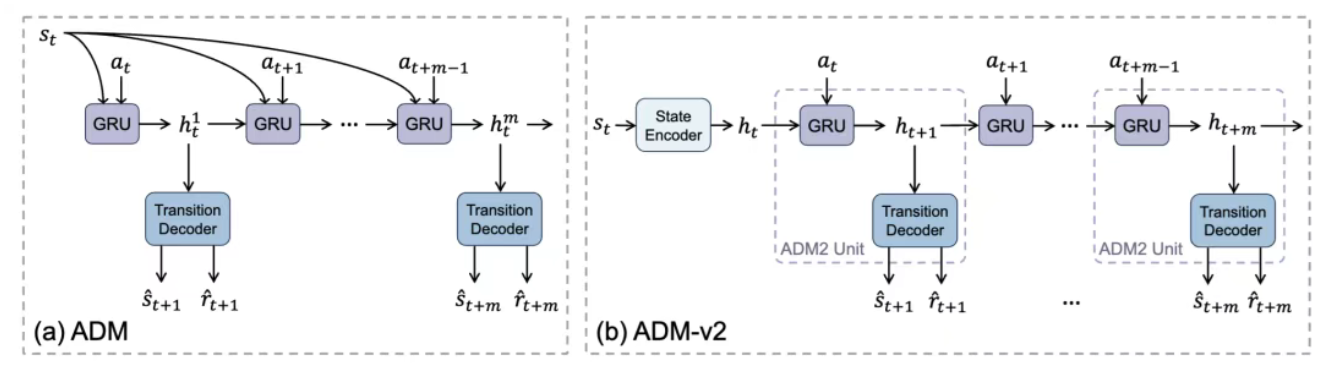
\includegraphics{images/image-0052.png}
\caption{GigaWorld-Policy 的训练与推理数据配方}
\end{figure}

\hypertarget{ux53c2ux8003ux6587ux732e-162}{%
\subsection{参考文献}\label{ux53c2ux8003ux6587ux732e-162}}

\vspace{0.25em}
\begin{itemize}
\tightlist
\item
  Open X-Embodiment Collaboration. (2023). \href{https://arxiv.org/abs/2310.08864}{Open X-Embodiment: Robotic Learning Datasets and RT-X Models}. arXiv:2310.08864.
\item
  Khazatsky, A., Pertsch, K., Nair, S., et al.~(2024). \href{https://arxiv.org/abs/2403.12945}{DROID: A Large-Scale In-The-Wild Robot Manipulation Dataset}. arXiv:2403.12945.
\item
  Chi, C., Xu, Z., Pan, C., et al.~(2024). \href{https://arxiv.org/abs/2402.10329}{Universal Manipulation Interface: In-The-Wild Robot Teaching Without In-The-Wild Robots}. arXiv:2402.10329.
\item
  Xu, M., Zhang, H., Hou, Y., et al.~(2025). \href{https://arxiv.org/abs/2505.21864}{DexUMI: Using Human Hand as the Universal Manipulation Interface for Dexterous Manipulation}. arXiv:2505.21864.
\item
  X Square Robot. (2026). \href{https://x2robot.com/en/pages/twindex}{TwinDEX --- Dexterous. Consistent. Scalable}. Project page.
\item
  Zheng, R., Niu, D., Xie, Y., et al.~(2026). \href{https://arxiv.org/abs/2602.16710}{EgoScale: Scaling Dexterous Manipulation with Diverse Egocentric Human Data}. arXiv:2602.16710.
\item
  Ye, A., Wang, B., Ni, C., et al.~(2026). \href{https://arxiv.org/abs/2603.17240}{GigaWorld-Policy: An Efficient Action-Centered World-Action Model}. arXiv:2603.17240.
\end{itemize}

\clearpage

\hypertarget{umiux6570ux636e}{%
\section{UMI数据}\label{umiux6570ux636e}}

\hypertarget{ux4e00umiux7684ux6838ux5fc3ux65b9ux6cd5}{%
\subsection{一、UMI的核心方法}\label{ux4e00umiux7684ux6838ux5fc3ux65b9ux6cd5}}

UMI用一个GoPro进行数据采集，包括一只手持夹爪及腕部视角相机，还通过两侧的镜子提供立体信息。UMI旨在用人类手持夹爪进行操作的方式采集数据，从而既具备人类操作的灵活性，又与机器人操作同构且本体无关，还可以让数据采集不再局限在封闭的数采厂，使得数据多样化程度更高、获取成本更低。

\begin{figure}[htbp]
\centering
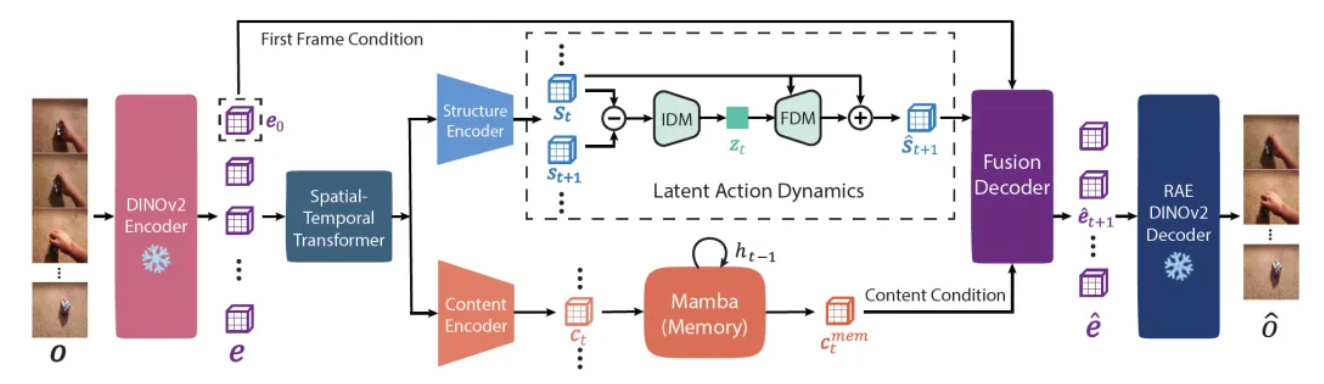
\includegraphics{images/image-0053.png}
\caption{UMI 手持数据采集设备}
\end{figure}

UMI采集的数据包括相机拍摄的图像、夹爪开合度（连续而非离散）以及相对末端执行器的位姿轨迹的数据。其中，图像采用腕部第一视角相机作为唯一的观测点；相对位姿表示解除了对特定机器人基坐标系的依赖，实现了本体无关性，用于机器人时只需将相对轨迹转化为关节指令即可。

\hypertarget{ux4e8cumiux6570ux636eux91c7ux96c6ux7684ux6539ux8fdbux4e0eux8d28ux91cfux63a7ux5236}{%
\subsection{二、UMI数据采集的改进与质量控制}\label{ux4e8cumiux6570ux636eux91c7ux96c6ux7684ux6539ux8fdbux4e0eux8d28ux91cfux63a7ux5236}}

\hypertarget{ux4e00umiux8bbeux5907ux7684ux6539ux8fdbux65b9ux5411}{%
\subsubsection{（一）UMI设备的改进方向}\label{ux4e00umiux8bbeux5907ux7684ux6539ux8fdbux65b9ux5411}}

\begin{enumerate}
\def\labelenumi{\arabic{enumi}.}
\item
  制造工艺调整、轻量化、易用性提升和鲁棒性提升。
\item
  针对部分操作中相机视野被遮挡，导致部分精细操作数据不可用的问题，可增加更多视角，但需要注意处理好具身差异。
\item
  针对触觉和力的数据缺失的问题，可增加相应传感器。
\item
  末端从简单的平行夹爪演进到更通用、更灵巧的末端形态。
\end{enumerate}

\hypertarget{ux4e8cumiux6570ux636eux91c7ux96c6ux7684ux8d28ux91cfux63a7ux5236}{%
\subsubsection{（二）UMI数据采集的质量控制}\label{ux4e8cumiux6570ux636eux91c7ux96c6ux7684ux8d28ux91cfux63a7ux5236}}

大规模数据采集中，常出现无效数据，如操作速度过快，超出了机器臂的物理极限；或者将手伸到机械臂无法复现的位置，导致运动学逆解失败。有时数据中还有大量无意义的片段，如反复拿起又放下同一个物体、打开开关后却没有进行下一步操作等。数据质量控制非常重要。如能实现实时质量控制，则相较于采集完毕后统一进行质量检查将能减少许多浪费。

另外，数据的难点不在于单纯的获取，而在于让获取的数据能用于模型训练。这需要数据和模型协同进化，将采集的数据用于模型迭代，发现问题后及时调整优化数据采集策略。

\hypertarget{ux4e09genux7cfbux5217ux57faux4e8eumiux6570ux636eux9884ux8badux7ec3ux7684scaling-law}{%
\subsection{三、GEN系列：基于UMI数据预训练的Scaling Law}\label{ux4e09genux7cfbux5217ux57faux4e8eumiux6570ux636eux9884ux8badux7ec3ux7684scaling-law}}

Generalist的GEN系列模型利用大规模UMI数据进行具身原生预训练。从GEN-0的27万小时，到GEN-1的50万小时，再到GEN-1.5更大规模的数据，模型能力不断提升。

在GEN-0的预训练中，Generalist发现模型的表现与计算、数据和参数的关系可以体现Scaling Law：

\begin{figure}[htbp]
\centering
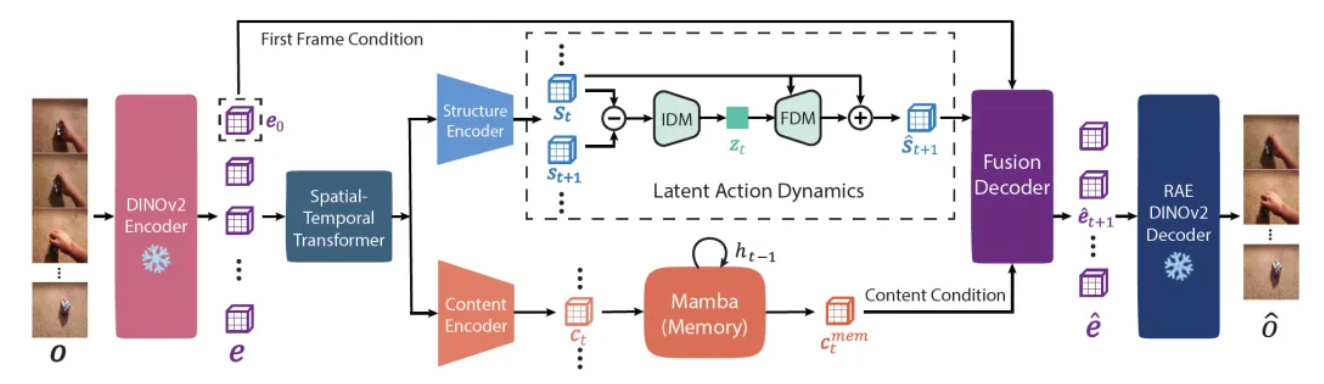
\includegraphics{images/image-0054.png}
\caption{GEN-0 随数据量和计算量扩展的性能曲线}
\end{figure}

\begin{figure}[htbp]
\centering
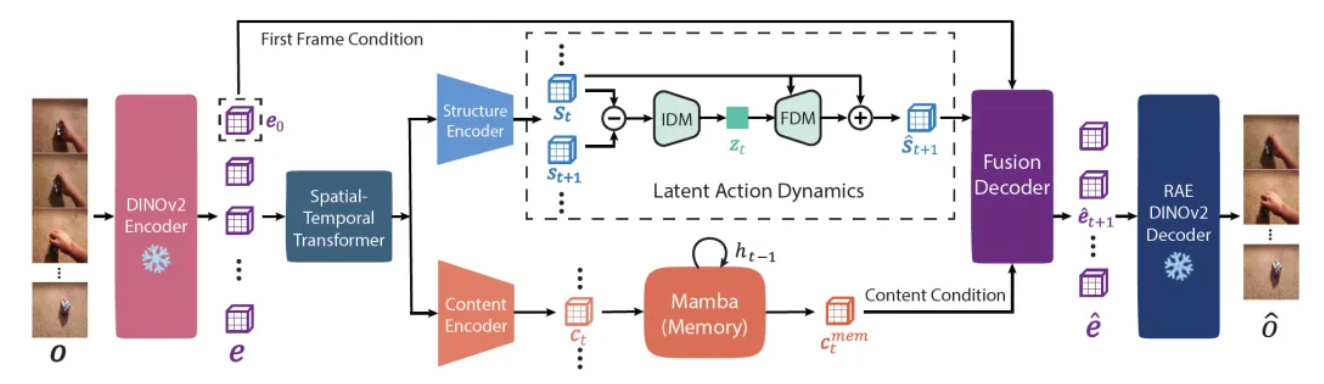
\includegraphics{images/image-0055.png}
\caption{GEN-0 随任务集合扩展的性能曲线}
\end{figure}

而到GEN-1.5，模型开始呈现出上下文学习能力。给模型看单次较短的示范，把它放进上下文窗口，机器人就能立刻做这件事，全程不需要更新梯度。仿真里录制的示范也可以（而GEN-1.5没有用仿真数据训练过）。物理提示可以像文本提示一样拼接，且模型可以通过类比的方式用示范里没有直接出现过的工具和策略进行操作。

如图是GEN-1.5预训练中损失持续呈下降趋势的曲线。

\begin{figure}[htbp]
\centering
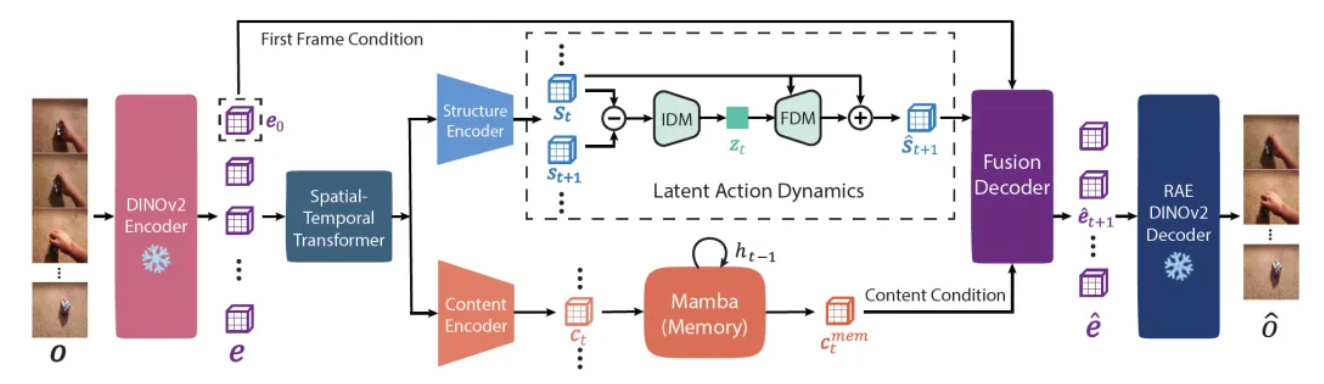
\includegraphics{images/image-0056.png}
\caption{GEN-1.5 的训练损失曲线}
\end{figure}

\hypertarget{ux56dbumiux7684ux884dux751fux4f53ux901aux8fc7ux53efux7a7fux6234ux5916ux9aa8ux9abcux91c7ux96c6ux6570ux636e}{%
\subsection{四、UMI的衍生体：通过可穿戴外骨骼采集数据}\label{ux56dbumiux7684ux884dux751fux4f53ux901aux8fc7ux53efux7a7fux6234ux5916ux9aa8ux9abcux91c7ux96c6ux6570ux636e}}

随着机器人末端从平行夹爪向多指灵巧手发展，UMI的思路也开始从手持夹爪进一步延伸到可穿戴外骨骼等。其核心仍然是利用人类直接操作真实物体来采集数据，但通过外骨骼将人的手部动作约束和映射到机器人灵巧手的可执行空间，从而减少人手与机器人手之间的具身差异。

以DexUMI为例，它为不同机器人灵巧手设计对应的手部外骨骼，使人可以直接完成抓取、旋拧、工具使用等复杂操作，同时记录多指动作和触觉信息。相比于先采集裸手动作再进行retargeting，外骨骼能够在数据采集阶段就缩小运动学差异。针对采集时看到``人手+外骨骼''、部署时看到机器人手所带来的视觉差异，DexUMI还通过视觉处理将采集画面转换得更接近机器人部署时的观测。

后续的一些工作也采用了类似思路，但进一步强调采集端与机器人端的协同设计。如TwinDEX的三指外骨骼与机器人三指手在运动学结构上尽可能保持一致，从硬件层面减少动作映射和retargeting的复杂度。数据采集设备正从简单夹爪向多指灵巧手发展，并越来越多地通过软硬件协同设计，在数据采集阶段就主动缩小Embodiment Gap。

\hypertarget{ux53c2ux8003ux6587ux732e-163}{%
\subsection{参考文献}\label{ux53c2ux8003ux6587ux732e-163}}

\vspace{0.25em}
\begin{itemize}
\tightlist
\item
  Chi, C., Xu, Z., Pan, C., et al.~(2024). \href{https://arxiv.org/abs/2402.10329}{Universal Manipulation Interface: In-The-Wild Robot Teaching Without In-The-Wild Robots}. arXiv:2402.10329.
\item
  Rayyan, O., Abanes, J., Hafez, M., Tzes, A., \& Abu-Dakka, F. (2025). \href{https://arxiv.org/abs/2509.18757}{MV-UMI: A Scalable Multi-View Interface for Cross-Embodiment Learning}. arXiv:2509.18757.
\item
  Liu, F., Li, C., Qin, Y., Xu, J., Abbeel, P., \& Chen, R. (2025). \href{https://arxiv.org/abs/2504.06156}{ViTaMIn: Learning Contact-Rich Tasks Through Robot-Free Visuo-Tactile Manipulation Interface}. arXiv:2504.06156.
\item
  Xu, M., Zhang, H., Hou, Y., et al.~(2025). \href{https://arxiv.org/abs/2505.21864}{DexUMI: Using Human Hand as the Universal Manipulation Interface for Dexterous Manipulation}. arXiv:2505.21864.
\item
  X Square Robot. (2026). \href{https://x2robot.com/en/pages/twindex}{TwinDEX --- Dexterous. Consistent. Scalable}. Project page.
\item
  Lin, F., Hu, Y., Sheng, P., Wen, C., You, J., \& Gao, Y. (2025). \href{https://proceedings.iclr.cc/paper_files/paper/2025/hash/88b7b2c896506daabc8d3fd587055167-Abstract-Conference.html}{Data Scaling Laws in Imitation Learning for Robotic Manipulation}. ICLR.
\item
  Generalist Team. (2025). \href{https://generalistai.com/blog/gen-0}{GEN-0: Embodied Foundation Models That Scale with Physical Interaction}. Generalist.
\item
  Generalist Team. (2026). \href{https://generalistai.com/blog/gen-1}{GEN-1: Scaling Embodied Foundation Models to Mastery}. Generalist.
\item
  Generalist Team. (2026). \href{https://generalistai.com/blog/gen-1.5}{GEN-1.5: Embodied Foundation Models are One-Shot Learners}. Generalist.
\end{itemize}

\clearpage

\hypertarget{ux4ebaux7c7bux7b2cux4e00ux89c6ux89d2ux6570ux636e}{%
\section{人类第一视角数据}\label{ux4ebaux7c7bux7b2cux4e00ux89c6ux89d2ux6570ux636e}}

\hypertarget{ux4e00ux4ebaux7c7bux7b2cux4e00ux89c6ux89d2ux89c6ux9891ux6570ux636eux6982ux8ff0}{%
\subsection{一、人类第一视角视频数据概述}\label{ux4e00ux4ebaux7c7bux7b2cux4e00ux89c6ux89d2ux89c6ux9891ux6570ux636eux6982ux8ff0}}

人类第一视角视频数据是具身智能模型的一类重要的训练数据。既可以规模化采集，又与具身操作的需求相契合。2026年起，从英伟达的EgoScale、DreamDojo到Dyna Robotics的Dyna-2，人类第一视角数据开始成为具身智能模型大规模预训练的一大数据来源。以EgoScale的训练过程为例：

\begin{figure}[htbp]
\centering
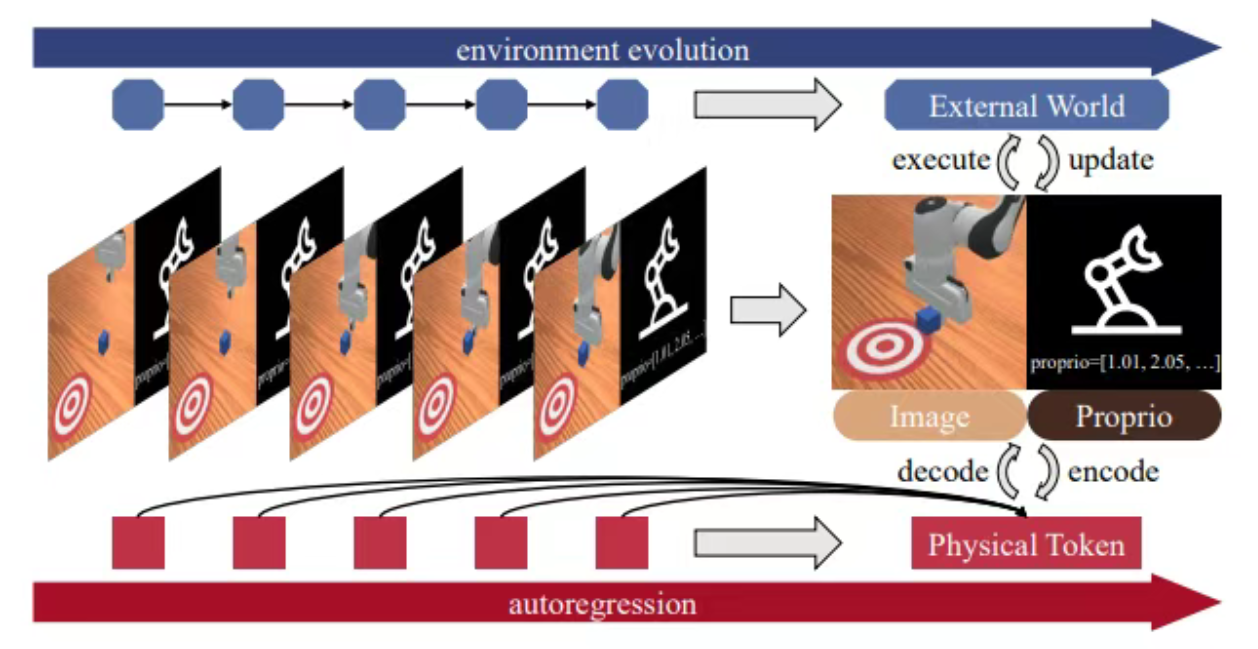
\includegraphics{images/image-0057.png}
\caption{EgoScale从人类第一视角视频预训练、人机对齐中期训练到灵巧任务后训练的流程}
\end{figure}

先在20,854小时人类第一视角视频上进行预训练，再用少量human-robot对齐数据做mid-training，最后进入具体的任务后训练。EgoScale标志着人类第一视角视频数据成为具身预训练Scaling的核心范式之一。

\hypertarget{ux4e8cux6a21ux578bux53efux4ee5ux4eceux4ebaux7c7bux7b2cux4e00ux89c6ux89d2ux89c6ux9891ux91ccux5b66ux4e60ux4ec0ux4e48ux4fe1ux53f7}{%
\subsection{二、模型可以从人类第一视角视频里学习什么信号？}\label{ux4e8cux6a21ux578bux53efux4ee5ux4eceux4ebaux7c7bux7b2cux4e00ux89c6ux89d2ux89c6ux9891ux91ccux5b66ux4e60ux4ec0ux4e48ux4fe1ux53f7}}

\hypertarget{ux4e00ux8868ux5f81ux5b66ux4e60ux538bux7f29}{%
\subsubsection{（一）表征学习（压缩）}\label{ux4e00ux8868ux5f81ux5b66ux4e60ux538bux7f29}}

\begin{enumerate}
\def\labelenumi{\arabic{enumi}.}
\item
  显式：如ATM（Any-point Trajectory Modeling）从人类视频中提取手和关键物体在图像平面上的二维显式运动路径，可作为关键点序列提供给策略网络；EgoVLA利用第一视角人类视频中显式提取的手部三维姿态和腕部轨迹作为预训练信号。
\item
  隐式：如LAPA不预定义中间变量语义，训练编码器把帧间变化压缩成低维的latent action隐式表征。
\end{enumerate}

\begin{figure}[htbp]
\centering
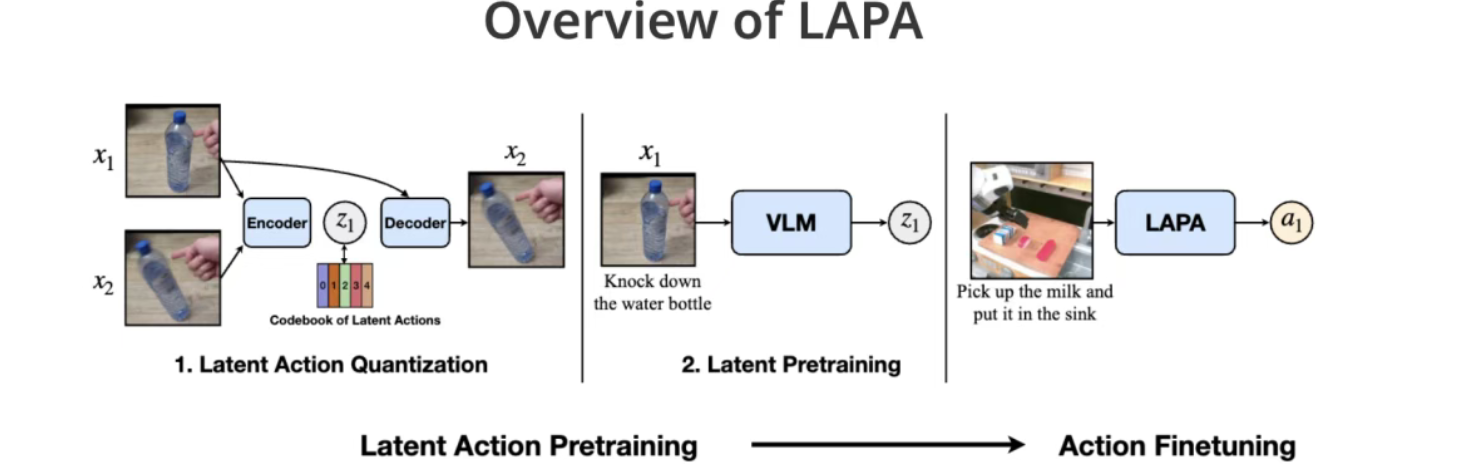
\includegraphics{images/image-0058.png}
\caption{LAPA潜在动作量化、潜在预训练与动作微调流程}
\end{figure}

\hypertarget{ux4e8cux4e16ux754cux6a21ux578bux5b66ux4e60ux9884ux6d4bux672aux6765}{%
\subsubsection{（二）世界模型学习（预测未来）}\label{ux4e8cux4e16ux754cux6a21ux578bux5b66ux4e60ux9884ux6d4bux672aux6765}}

\begin{enumerate}
\def\labelenumi{\arabic{enumi}.}
\item
  显式：字节跳动的GR-1用人类第一视角视频训练视频生成模型，让模型在给定当前帧和语言指令的情况下预测未来帧，后续迁移到机器人场景后，相比纯robot data baseline有显著提升，从而证明了人类第一视角视频里有助于具身智能模型的训练。
\item
  隐式：以DreamDojo为例，在隐空间中同时学习下一状态预测和动作预测。
\end{enumerate}

\hypertarget{ux4e09ux4eceux4ebaux7c7bux5230ux673aux5668ux4ebaux7684ux8fc1ux79fb}{%
\subsection{三、从人类到机器人的迁移}\label{ux4e09ux4eceux4ebaux7c7bux5230ux673aux5668ux4ebaux7684ux8fc1ux79fb}}

具身智能模型最终要生成的是动作，而人类第一视角数据并不自带动作。而且，人类与机器人存在Embodiment Gap，人手的自由度和机械臂不同，运动空间也不完全同构。因此，人类第一视角视频数据在用于机器人模型的预训练前，要通过一些方法进行处理，才能实现数据的跨本体迁移。下面介绍几种方法。

具身智能模型最终需要输出机器人动作，但人类第一视角视频通常不带机器人动作标签，而且人手、机械臂、灵巧手等本体在自由度、关节结构和运动空间上并不一致，因此存在明显的 Embodiment Gap。要让人类视频用于机器人预训练，通常需要先进行跨本体处理。现有方法大致可以分为以下四类。

\hypertarget{ux4e00ux6539ux5199ux6570ux636eux672cux8eabux7684ux89c6ux89c9ux5916ux89c2ux7f29ux5c0fux4ebaux4e0eux673aux5668ux4ebaux89c2ux6d4bux5deeux5f02}{%
\subsubsection{（一）改写数据本身的视觉外观，缩小人与机器人观测差异}\label{ux4e00ux6539ux5199ux6570ux636eux672cux8eabux7684ux89c6ux89c9ux5916ux89c2ux7f29ux5c0fux4ebaux4e0eux673aux5668ux4ebaux89c2ux6d4bux5deeux5f02}}

这类方法主要解决人和机器人``看起来不同''的问题。其核心是修改图像，使人类视频和机器人观测在视觉分布上更加接近。

例如，Phantom、Qwen-RobotManip先移除图像中的人手，再根据原来人手的运动轨迹，在物理仿真中计算机器人机械臂应该如何运动，然后在图像的相同位置叠加虚拟机器人；推理时也对真实机器人观测进行同样处理，以保持训练和部署输入一致。EgoMimic则使用SAM掩蔽人手和机械臂，并用统一的红色线条表示手或末端执行器方向，从而弱化本体外观差异，让模型更多关注物体、接触区域和操作方向。

\begin{figure}[htbp]
\centering
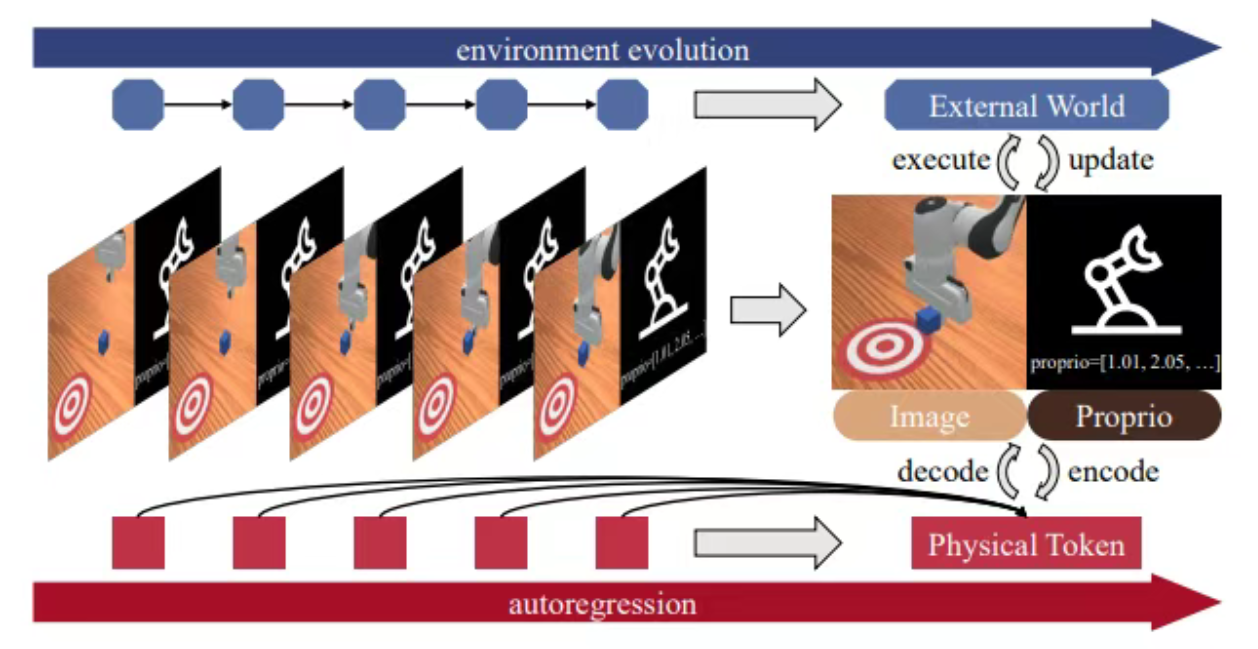
\includegraphics{images/image-0059.png}
\caption{EgoMimic掩蔽前的人手与机器人观测}
\end{figure}

\begin{figure}[htbp]
\centering
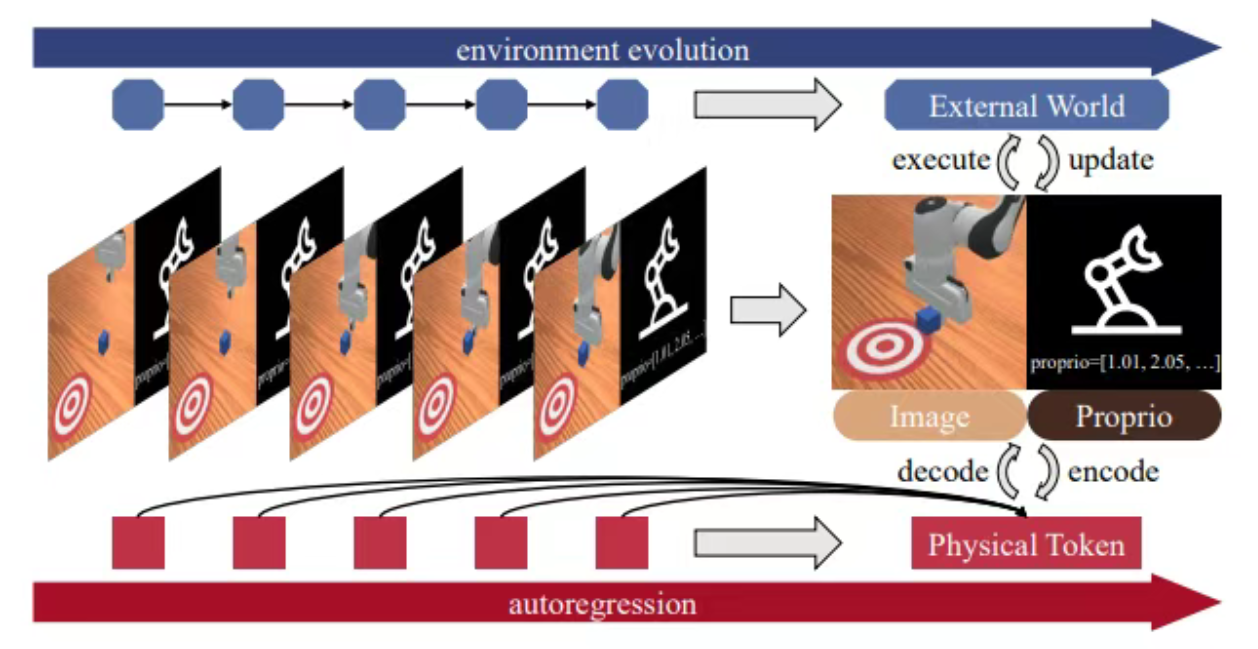
\includegraphics{images/image-0060.png}
\caption{EgoMimic掩蔽后以红色线条统一表示操作方向}
\end{figure}

这类方法主要解决Observation Gap，本身并没有把人的动作转换成机器人动作，因此通常需要与后续动作对齐方法结合。

\hypertarget{ux4e8cux5c06ux4ebaux7684ux52a8ux4f5cux663eux5f0fux6620ux5c04ux4e3aux673aux5668ux4ebaux52a8ux4f5c}{%
\subsubsection{（二）将人的动作显式映射为机器人动作}\label{ux4e8cux5c06ux4ebaux7684ux52a8ux4f5cux663eux5f0fux6620ux5c04ux4e3aux673aux5668ux4ebaux52a8ux4f5c}}

这类方法直接建立``人类动作→机器人动作''的映射关系。通常先从视频中恢复人的手腕、手指或三维关键点轨迹，再通过坐标变换、逆运动学、retargeting或轨迹优化，得到机器人可执行动作。

例如，DexMV先用MANO恢复人手三维姿态，再通过运动学优化将人手动作映射到机器人灵巧手关节空间。机械臂任务中也可以将人的wrist pose转成机器人末端执行器目标位姿，再通过IK求解机器人关节动作。

这一方法物理意义明确，但扩展性较差。因为不同机器人结构不同，往往需要分别设计 Human→Robot A、Human→Robot B等映射，难以扩展到大量异构机器人。

\hypertarget{ux4e09ux8bbeux8ba1ux4ebaux548cux673aux5668ux4ebaux5171ux4eabux7684ux52a8ux4f5cux8868ux793a}{%
\subsubsection{（三）设计人和机器人共享的动作表示}\label{ux4e09ux8bbeux8ba1ux4ebaux548cux673aux5668ux4ebaux5171ux4eabux7684ux52a8ux4f5cux8868ux793a}}

这类方法不再直接把人的动作翻译成某一种机器人动作，而是另外设计一个所有本体都可以使用的共享动作空间，无论人类动作还是机器人A、机器人B，都映射到共享动作空间。

也就是说，不再为每一对本体单独设计动作映射，而是让不同本体使用同一种``动作语言''。

以Being-H0.5为例，它构造了统一的State-Action Space，将动作向量划分为具有明确物理意义的不同维度或槽位，例如：

\begin{enumerate}
\def\labelenumi{\arabic{enumi}.}
\item
  末端执行器平移：表示手腕或机器人末端执行器在 x,y,zx,y,z 方向上的运动。
\item
  末端执行器旋转：表示手腕或末端执行器的姿态变化。
\item
  机械臂关节状态/动作：表示机器人各关节的位置或运动。
\item
  手指动作：表示人手或灵巧手的精细手指运动。
\item
  夹爪开合：表示两指夹爪等末端机构的开闭状态。
\item
  移动底盘动作：表示移动机器人的平移、转向等运动。
\end{enumerate}

不同本体只使用与自身有关的维度。例如，人类数据可以用wrist pose填入末端执行器相关维度，用MANO手指参数表示精细操作；机械臂机器人可以使用末端执行器和机械臂关节维度；灵巧手机器人则额外使用手指动作维度；移动操作机器人还可以使用底盘动作维度。因此，不同本体虽然自由度不同，但具有相同物理意义的动作被放在统一位置。模型可以在人类视频和多种机器人数据上联合训练，共享``向前移动''``旋转手腕''``接近物体''``抓取''等跨本体的运动规律。

Dyna-2则是另一种案例，它没有刻意设计很多不同维度或槽位，而是从数据中恢复三维手部轨迹后，把复杂的人手运动仅压缩为两类维度：

\begin{enumerate}
\def\labelenumi{\arabic{enumi}.}
\item
  腕部姿态：对应机器人的末端执行器运动。
\item
  拇指-食指开合：对应机器人的gripper开合。
\end{enumerate}

这种``极简''的设计只对共享动作表示作了最基本的规定，没有通过任何视觉或本体相关的数据处理来缩小预训练数据与机器人数据之间的视觉或运动学差距，事实上是给模型``留出空间''，把迁移的能力交由大规模世界-动作模型预训练来实现，通过大量数据训练世界模型来学习跨本体共享的物理动态。

当然，为了提高跨本体的可迁移性，我们可以不直接提取机器人具体哪个关节应该运动多少的信息，而是提取更高层、更加本体无关的操作知识，例如接触点、抓取姿态、物体可供性和手物交互模式等，如MAPLE从Ego4D中学习手与物体的接触位置以及接触时的三维手部姿态。这些信息告诉机器人``应该在哪里接触''``应该以什么方式抓取''等。接触点、抓取区域和affordance等知识通常比精确关节轨迹更加本体无关。

\hypertarget{ux56dbux901aux8fc7ux8f6fux786cux4ef6ux534fux540cux8bbeux8ba1ux4f7fux673aux5668ux4ebaux672cux4f53ux4e3bux52a8ux5bf9ux9f50ux4ebaux7c7b}{%
\subsubsection{（四）通过软硬件协同设计，使机器人本体主动对齐人类}\label{ux56dbux901aux8fc7ux8f6fux786cux4ef6ux534fux540cux8bbeux8ba1ux4f7fux673aux5668ux4ebaux672cux4f53ux4e3bux52a8ux5bf9ux9f50ux4ebaux7c7b}}

前三类方法基本都默认机器人本体已经确定，再通过视觉处理、动作映射或表示学习跨越人与机器人之间的Embodiment Gap。这类方法则反过来思考：与其不断设计更复杂的算法让人类数据适配机器人，不如在机器人设计阶段就主动向人类的身体结构、动作空间和感知方式对齐，从源头缩小Embodiment Gap。

Human-as-Humanoid是这一思路的典型例子。其核心不是取消动作转换，而是通过软硬件协同设计，将原本复杂的跨本体迁移问题简化为相对直接的运动学映射。为此，PrimeU在多个层面按照人类操作方式设计：

\begin{enumerate}
\def\labelenumi{\arabic{enumi}.}
\item
  身体比例对齐：肩宽、臂长和关节活动范围接近成年人，使人和机器人的可达空间尽量一致。
\item
  自由度对齐：两条7自由度机械臂、两只各20自由度灵巧手，再加3自由度颈部和3自由度腰部，共60自由度，尽可能覆盖人类上半身和手部的主要运动能力。
\item
  手部结构对齐：灵巧手自由度按照人手运动学结构分布，使捏、握、旋转等人类操作可以较直接地对应到机器人。
\item
  感知视角对齐：机器人头部和手腕布置摄像头，人类数据采集也采用对应的第一视角和手部附近视角，从而缩小训练和部署时的视觉差异。
\end{enumerate}

在这种硬件基础上，人类视频到机器人动作的转换可以采用较简单的流程：

人类ego/exo视频→人体与手部关键点→分阶段IK→60自由度机器人动作。

其中，第一视角视频直接作为模型的视觉输入，第三视角视频用于恢复人体运动；随后通过 Staged IK 依次求解手部、手臂与手腕、颈部和腰部动作，再进行关节限位和平滑处理。由于机器人的比例、自由度和运动范围已经主动向人体对齐，这里的retargeting不再需要解决严重的跨形态差异，而主要成为一个运动学求解问题。

在模型训练阶段，Human-as-Humanoid还通过DS-HKC（Dual-Space Hierarchical Kinematic Consistency） 同时约束关节空间和任务空间。模型预测的60维关节动作不仅要接近转换得到的关节标签，还要经过正向运动学后，使手腕、指尖等关键位置与原始动作保持一致，从而避免高自由度系统中``关节角合理，但实际手部位置偏移''的问题。

\hypertarget{ux56dbdyna-2ux4ebaux7c7bux7b2cux4e00ux89c6ux89d2ux89c6ux9891ux6570ux636eux4e0aux7684scaling-law}{%
\subsection{四、Dyna-2：人类第一视角视频数据上的Scaling Law}\label{ux56dbdyna-2ux4ebaux7c7bux7b2cux4e00ux89c6ux89d2ux89c6ux9891ux6570ux636eux4e0aux7684scaling-law}}

Dyna-2运用人类第一视角视频数据进行预训练。其技术报告指出，当人类第一视角视频数据从1000小时扩展到100万小时，可观察到多方面的Scaling Law。

\hypertarget{ux4e00ux4ebaux7c7bux6570ux636eux9a8cux8bc1ux96c6ux4e0aux7684ux52a8ux4f5cux9884ux6d4bux6548ux679cux968fux9884ux8badux7ec3ux6570ux636eux91cfux7684ux53d8ux5316}{%
\subsubsection{（一）人类数据验证集上的动作预测效果随预训练数据量的变化}\label{ux4e00ux4ebaux7c7bux6570ux636eux9a8cux8bc1ux96c6ux4e0aux7684ux52a8ux4f5cux9884ux6d4bux6548ux679cux968fux9884ux8badux7ec3ux6570ux636eux91cfux7684ux53d8ux5316}}

\begin{figure}[htbp]
\centering
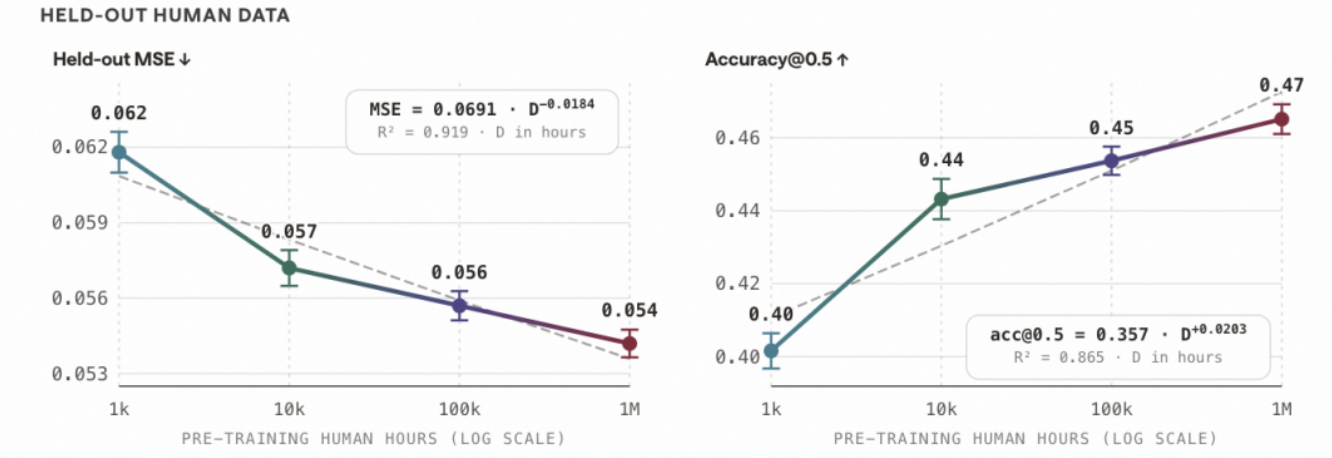
\includegraphics{images/image-0061.png}
\caption{Dyna-2在留出人类数据上随预训练时数增长的误差与准确率曲线}
\end{figure}

可以看出，随着人类数据量的不断扩展，模型的损失下降和准确率上升基本符合幂律 \(y=a\cdot D^{-b}\)（图中虚线）。

\hypertarget{ux4e8cux96f6ux6837ux672cux673aux5668ux4ebaux6570ux636eux96c6ux4e0aux7684ux52a8ux4f5cux9884ux6d4bux6548ux679cux968fux9884ux8badux7ec3ux6570ux636eux91cfux7684ux53d8ux5316}{%
\subsubsection{（二）零样本机器人数据集上的动作预测效果随预训练数据量的变化}\label{ux4e8cux96f6ux6837ux672cux673aux5668ux4ebaux6570ux636eux96c6ux4e0aux7684ux52a8ux4f5cux9884ux6d4bux6548ux679cux968fux9884ux8badux7ec3ux6570ux636eux91cfux7684ux53d8ux5316}}

\begin{figure}[htbp]
\centering
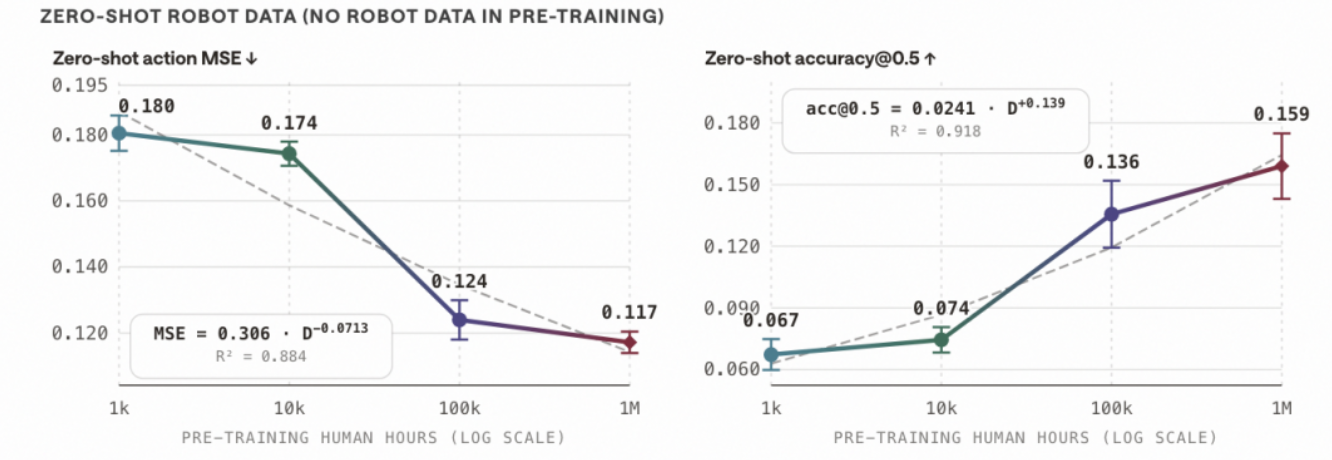
\includegraphics{images/image-0062.png}
\caption{Dyna-2仅用人类数据预训练后在零样本机器人数据上的误差与准确率曲线}
\end{figure}

仅在人类数据上预训练后，直接在留出的机器人数据上评测，依然呈现出跨越本体鸿沟的规模化定律：随着纯人类数据增长，机器人验证指标单调下降。

\hypertarget{ux4e09ux5faeux8c03ux540eux771fux673aux9a8cux8bc1ux6548ux679cux968fux9884ux8badux7ec3ux6570ux636eux91cfux7684ux53d8ux5316}{%
\subsubsection{（三）微调后真机验证效果随预训练数据量的变化}\label{ux4e09ux5faeux8c03ux540eux771fux673aux9a8cux8bc1ux6548ux679cux968fux9884ux8badux7ec3ux6570ux636eux91cfux7684ux53d8ux5316}}

\begin{figure}[htbp]
\centering
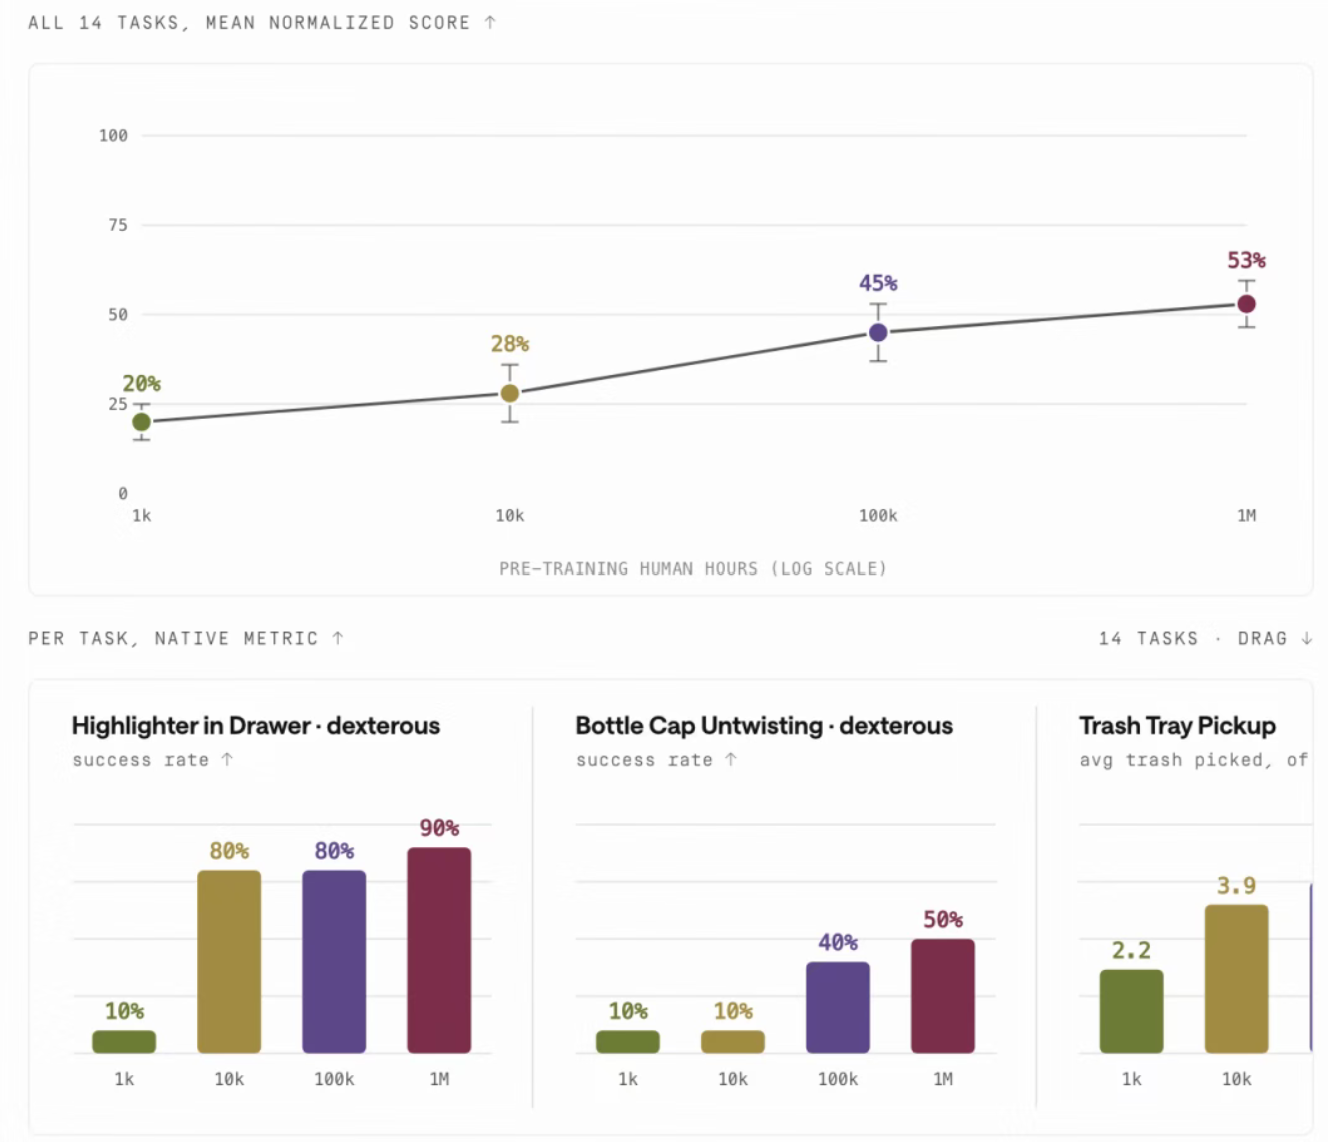
\includegraphics{images/image-0063.png}
\caption{Dyna-2不同预训练数据规模下微调后的真机任务表现}
\end{figure}

预训练的规模化定律可以跨越任务、本体与能力，在微调后的真机上呈现。

\hypertarget{ux56dbux4e16ux754cux5efaux6a21ux662fux8de8ux672cux4f53ux89c4ux6a21ux5316ux5b9aux5f8bux6d8cux73b0ux7684ux5173ux952e}{%
\subsubsection{（四）世界建模是跨本体规模化定律涌现的关键}\label{ux56dbux4e16ux754cux5efaux6a21ux662fux8de8ux672cux4f53ux89c4ux6a21ux5316ux5b9aux5f8bux6d8cux73b0ux7684ux5173ux952e}}

Dyna-2同时学习预测未来世界状态和动作。作者通过受控实验发现，真正推动跨本体迁移随数据规模增长而提升的关键，不是单纯扩大动作数据，而是引入世界建模，尤其是未来视频预测。实验种，固定带手部姿态标注的人类动作数据量（5k、50k、100k 小时），使用相同模型架构比较三种训练方式：

Action-only：只预测动作，不进行世界建模。

Joint：同时预测动作和未来视频。

Video co-training：在Joint基础上，再加入等量、无动作标签的人类视频，仅用于未来视频预测。

三种模型均在39个机器人任务上进行零样本评测。结果显示，Joint在所有数据规模上都优于Action-only，说明未来预测本身能够显著改善跨本体迁移；但随着动作数据继续增加，Action-only容易出现明显过拟合，Joint的性能也没有持续随规模提升。只有加入大量纯视频数据的Video co-training，性能才随着数据规模稳定增长。进一步地，在分别固定50k和250k 小时带动作标签的人类数据，只增加无动作标签的视频数据规模，仍能使机器人留出集上的泛化性能单调提升。因此，如果希望利用大规模人类视频实现human-to-robot transfer，世界建模可能才是弥合本体差异的关键因素。

\begin{figure}[htbp]
\centering
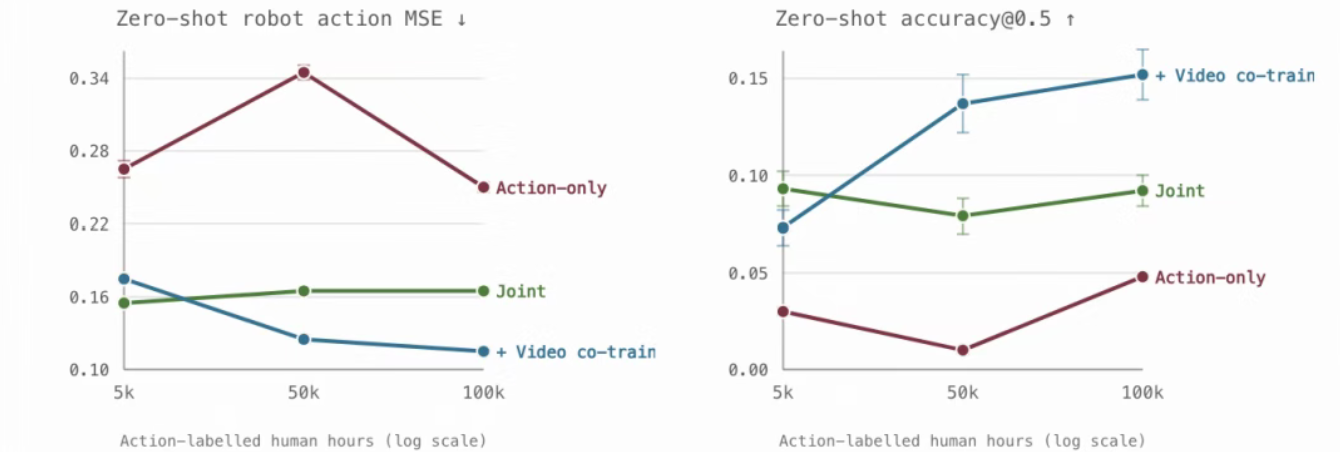
\includegraphics{images/image-0064.png}
\caption{Dyna-2动作预测、联合训练与视频协同训练的零样本机器人消融实验}
\end{figure}

值得注意的是，扩展纯视频数据并不会明显提高模型在人类同本体动作数据上的表现，甚至可能略有下降。这说明视频建模的主要价值可能不在于提升同本体动作拟合，而更多在于帮助模型学习更一般的物体运动、接触关系和物理动态，从而提升对未见机器人本体的迁移能力。

\hypertarget{ux4e94ux89c6ux9891ux9884ux8badux7ec3ux53efux80fdux5e26ux6765ux6307ux4ee4ux8ddfux968fux80fdux529bux7684ux63d0ux5347}{%
\subsubsection{（五）视频预训练可能带来指令跟随能力的提升}\label{ux4e94ux89c6ux9891ux9884ux8badux7ec3ux53efux80fdux5e26ux6765ux6307ux4ee4ux8ddfux968fux80fdux529bux7684ux63d0ux5347}}

Dyna-2的技术报告还提出，视频预测本身带来了指令跟随能力的提升。作者设计了四类反事实语言任务，包括按指令推或拉积木，从多个物体中选择指定目标并放入盒中，按语言要求改变积木堆叠顺序，以及对餐巾执行拿起、拉动、旋转、翻面、折叠、抚平等多种操作。评测时保持视觉场景基本不变，只改变语言指令，从而检验模型是否真正根据语言选择动作。

结果显示，从action-only切换到视频联合训练后，总体成功率显著提升；进一步使用更大规模视频预料进行视频联合训练后，成功率进一步大幅提升，其中物体指代和复杂动作原语的提升最明显。这些结果表明，更大、更丰富的视频数据和世界建模不仅提升跨本体泛化，可能也可以通过帮助模型学习``语言---物体---动作---物理结果''之间的对应关系，增强模型的语言指令跟随能力。

\hypertarget{ux53c2ux8003ux6587ux732e-164}{%
\subsection{参考文献}\label{ux53c2ux8003ux6587ux732e-164}}

\vspace{0.25em}
\begin{itemize}
\tightlist
\item
  具身纪元. (2026). \href{https://www.jintiankansha.com/t/rxSAsq869K}{硅谷大火的ego数据，正改写具身数据新规则}. 微信公众号文章，2026年3月17日发布.
\item
  具身纪元. (2026). \href{https://www.jintiankansha.com/t/PtzdfzjSA4}{我们之前利用人类视频数据的方法，可能都走错了方向}. 微信公众号文章，2026年7月8日发布.
\item
  Damen, D., Doughty, H., Farinella, G. M., et al.~(2018). \href{https://arxiv.org/abs/1804.02748}{Scaling Egocentric Vision: The EPIC-KITCHENS Dataset}. ECCV.
\item
  Grauman, K., Westbury, A., Byrne, E., et al.~(2022). \href{https://arxiv.org/abs/2110.07058}{Ego4D: Around the World in 3,000 Hours of Egocentric Video}. CVPR.
\item
  Zheng, R., Niu, D., Xie, Y., et al.~(2026). \href{https://arxiv.org/abs/2602.16710}{EgoScale: Scaling Dexterous Manipulation with Diverse Egocentric Human Data}. arXiv:2602.16710.
\item
  Gao, S., Liang, W., Zheng, K., et al.~(2026). \href{https://arxiv.org/abs/2602.06949}{DreamDojo: A Generalist Robot World Model from Large-Scale Human Videos}. arXiv:2602.06949.
\item
  Dyna Robotics. (2026). \href{https://www.dyna.co/dyna-2}{Dyna-2: A 1-Million-Hour Scaling Law for World-Action Models}. Technical report, August 2026.
\item
  Nair, S., Rajeswaran, A., Kumar, V., Finn, C., \& Gupta, A. (2022). \href{https://arxiv.org/abs/2203.12601}{R3M: A Universal Visual Representation for Robot Manipulation}. Conference on Robot Learning.
\item
  Ma, Y. J., Sodhani, S., Jayaraman, D., Bastani, O., Kumar, V., \& Zhang, A. (2023). \href{https://arxiv.org/abs/2210.00030}{VIP: Towards Universal Visual Reward and Representation via Value-Implicit Pre-Training}. ICLR.
\item
  Wen, C., Lin, X., So, J. I. R., et al.~(2024). \href{https://www.roboticsproceedings.org/rss20/p092.html}{Any-point Trajectory Modeling for Policy Learning}. Robotics: Science and Systems. https://doi.org/10.15607/RSS.2024.XX.092.
\item
  Yang, R., Yu, Q., Wu, Y., et al.~(2025). \href{https://arxiv.org/abs/2507.12440}{EgoVLA: Learning Vision-Language-Action Models from Egocentric Human Videos}. arXiv:2507.12440.
\item
  Ye, S., Jang, J., Jeon, B., et al.~(2025). \href{https://openreview.net/forum?id=VYOe2eBQeh}{Latent Action Pretraining from Videos}. ICLR. arXiv:2410.11758.
\item
  Yang, J., Shi, Y., Zhu, H., et al.~(2025). \href{https://arxiv.org/abs/2505.17006}{CoMo: Learning Continuous Latent Motion from Internet Videos for Scalable Robot Learning}. arXiv:2505.17006.
\item
  Wu, H., Jing, Y., Cheang, C., et al.~(2024). \href{https://openreview.net/forum?id=NxoFmGgWC9}{Unleashing Large-Scale Video Generative Pre-training for Visual Robot Manipulation}. ICLR. arXiv:2312.13139.
\item
  Mendonca, R., Bahl, S., \& Pathak, D. (2023). \href{https://arxiv.org/abs/2308.10901}{Structured World Models from Human Videos}. Robotics: Science and Systems.
\item
  Lepert, M., Fang, J., \& Bohg, J. (2025). \href{https://proceedings.mlr.press/v305/lepert25a.html}{Phantom: Training Robots Without Robots Using Only Human Videos}. Conference on Robot Learning. arXiv:2503.00779.
\item
  Yuan, H., Liang, Z., Chen, A., et al.~(2026). \href{https://arxiv.org/abs/2606.17846}{Qwen-RobotManip Technical Report: Alignment Unlocks Scale for Robotic Manipulation Foundation Models}. arXiv:2606.17846.
\item
  Kareer, S., Patel, D., Punamiya, R., et al.~(2024). \href{https://arxiv.org/abs/2410.24221}{EgoMimic: Scaling Imitation Learning via Egocentric Video}. arXiv:2410.24221.
\item
  Kirillov, A., Mintun, E., Ravi, N., et al.~(2023). \href{https://openaccess.thecvf.com/content/ICCV2023/html/Kirillov_Segment_Anything_ICCV_2023_paper.html}{Segment Anything}. ICCV.
\item
  Qin, Y., Wu, Y.-H., Liu, S., et al.~(2022). \href{https://arxiv.org/abs/2108.05877}{DexMV: Imitation Learning for Dexterous Manipulation from Human Videos}. ECCV.
\item
  Romero, J., Tzionas, D., \& Black, M. J. (2017). \href{https://doi.org/10.1145/3130800.3130883}{Embodied Hands: Modeling and Capturing Hands and Bodies Together}. ACM Transactions on Graphics, 36(6), Article 245. (MANO)
\item
  Bahl, S., Gupta, A., \& Pathak, D. (2022). \href{https://arxiv.org/abs/2207.09450}{Human-to-Robot Imitation in the Wild}. Robotics: Science and Systems.
\item
  Singh, H. G., Loquercio, A., Sferrazza, C., et al.~(2025). \href{https://arxiv.org/abs/2409.08273}{Hand-Object Interaction Pretraining from Videos}. ICRA.
\item
  Luo, H., Wang, Y., Zhang, W., et al.~(2026). \href{https://arxiv.org/abs/2601.12993}{Being-H0.5: Scaling Human-Centric Robot Learning for Cross-Embodiment Generalization}. arXiv:2601.12993.
\item
  Gavryushin, A., Wang, X., Malate, R. J. S., et al.~(2025). \href{https://arxiv.org/abs/2504.06084}{MAPLE: Encoding Dexterous Robotic Manipulation Priors Learned From Egocentric Videos}. arXiv:2504.06084.
\item
  Cai, X., Qiu, R.-Z., Chen, G., et al.~(2025). \href{https://arxiv.org/abs/2511.15704}{In-N-On: Scaling Egocentric Manipulation with in-the-wild and on-task Data}. arXiv:2511.15704.
\item
  Li, Q., Deng, Y., Liang, Y., et al.~(2025). \href{https://arxiv.org/abs/2510.21571}{Scalable Vision-Language-Action Model Pretraining for Robotic Manipulation with Real-Life Human Activity Videos}. arXiv:2510.21571.
\item
  Yang, B., Li, Z., Sun, Y., et al.~(2026). \href{https://arxiv.org/abs/2602.23893}{AoE: Always-on Egocentric Human Video Collection for Embodied AI}. arXiv:2602.23893.
\item
  Lin, X., Yang, R., Lian, S., et al.~(2026). \href{https://arxiv.org/abs/2606.32009}{Human-as-Humanoid: Enabling Zero-Shot Humanoid Learning from Ego-Exo Human Videos with Human-Aligned Embodiments}. arXiv:2606.32009.
\item
  Feng, Z., Li, Q., Liang, H., et al.~(2026). \href{https://arxiv.org/abs/2606.00054}{From Human Videos to Robot Manipulation: A Survey on Scalable Vision-Language-Action Learning with Human-Centric Data}. IJCAI 2026 Survey Track.
\end{itemize}

\clearpage

\hypertarget{ux6570ux636eux7684ux5904ux7406ux4e0eux5bf9ux9f50}{%
\section{数据的处理与对齐}\label{ux6570ux636eux7684ux5904ux7406ux4e0eux5bf9ux9f50}}

对于具身智能的数据，除了规模和多样性之外，数据如何进行处理、如何与训练的需要对齐也非常值得注重。

\hypertarget{ux4e00ux3c00.7ux7528promptux5904ux7406ux6570ux636e}{%
\subsection{一、π0.7：用Prompt处理数据}\label{ux4e00ux3c00.7ux7528promptux5904ux7406ux6570ux636e}}

π0.7涌现出组合泛化能力的关键在于用多样化的prompt处理多样化的数据。过去VLA训练只喂一句清理冰箱，模型得到的信号是单一的。π0.7把prompt展开成四层：

\begin{enumerate}
\def\labelenumi{\arabic{enumi}.}
\item
  任务指令。例如，要清理厨房。
\item
  子任务指令。例如，要打开冰箱、取出食材、清理桌面等。
\item
  子目标图像，即``下一帧画面应该长什么样''。
\item
  episode元数据，即这条数据质量几分、有没有出错、速度多快等。
\end{enumerate}

有了这些丰富的context，模型就能分得清训练数据里的好坏、快慢、对错，从而可以用好以前用不了的数据，如失败的rollouts、低质量的演示、其他机器人的片段等。π0.7加的这层prompt，就是让模型知道``这段数据是什么质量、用什么策略做的''。

\hypertarget{ux4e8cqwen-robotmanipux6570ux636eux7684ux5bf9ux9f50}{%
\subsection{二、Qwen-RobotManip：数据的对齐}\label{ux4e8cqwen-robotmanipux6570ux636eux7684ux5bf9ux9f50}}

处理来自大量机器人和数据集的数据时，不能简单把它们收集到一起。比如，同样是``把杯子推到桌子边缘''这个动作，不同机器人记录它的方式可能完全不同。有的机器人记录7个关节分别转了多少角度；有的记录机械臂末端在机器人基座坐标系里的位置和姿态；还有一些灵巧手，本身就有二十多个可以独立运动的关节。这些数字虽然描述的是类似的动作，但它们并不是同一种``语言''。如果直接把它们混在一起训练，模型很难知道哪些变化其实代表同一个动作，最后往往会学到噪声。Qwen-RobotManip在多个层面对数据进行对齐和清晰，观察到模型的性能随着数据量的增大稳步提升。

\hypertarget{ux4e00ux4e0dux540cux6570ux636eux7684ux683cux5f0fux5bf9ux9f50}{%
\subsubsection{（一）不同数据的格式对齐}\label{ux4e00ux4e0dux540cux6570ux636eux7684ux683cux5f0fux5bf9ux9f50}}

\hypertarget{ux52a8ux4f5cux7ef4ux5ea6ux5b9aux4e49ux5bf9ux9f50}{%
\paragraph{1. 动作维度定义对齐}\label{ux52a8ux4f5cux7ef4ux5ea6ux5b9aux4e49ux5bf9ux9f50}}

不同机器人的身体结构差别很大。有单臂机器人，有双臂机器人；有普通夹爪，也有十几个甚至几十个自由度的灵巧手。它们原始的状态和动作维度完全不同。Qwen-RobotManip把机器人的状态和动作统一表示成一个80维向量，前58维均分给两条手臂，每条手臂内部关节位置7维、末端位姿9维、夹爪状态1维，灵巧手关节12维；后22维备用。某台机器人没有的部件，对应位置就补成0。

由于补出来的0并不是真实数据，模型会使用一个0-1二值掩码，以确定哪些维度是补0。训练时，只有真实存在的维度参与计算误差和更新梯度。

\hypertarget{ux5750ux6807ux7cfbux5bf9ux9f50}{%
\paragraph{2. 坐标系对齐}\label{ux5750ux6807ux7cfbux5bf9ux9f50}}

假设两台机器人都让机械臂向前移动10厘米，因为它们的底座安装位置、朝向和坐标定义不同，在各自的基座坐标系里，这个动作可能会变成完全不同的一组数字。故Qwen-RobotManip不直接使用原始坐标系里的绝对位置，而是更多地使用相机坐标系下的末端位姿变化量，避免了坐标系原点不同带来的麻烦。此外，模型还会获取关于摄像机安装位置、朝向以及末端执行器类型的信息。

\hypertarget{ux5728ux4e0aux4e0bux6587ux4e2dux63d0ux4f9bux5f53ux524dux673aux5668ux4ebaux7684ux7279ux5f81}{%
\paragraph{3. 在上下文中提供当前机器人的特征}\label{ux5728ux4e0aux4e0bux6587ux4e2dux63d0ux4f9bux5f53ux524dux673aux5668ux4ebaux7684ux7279ux5f81}}

前面讲到了如何让模型有效学习各种不同机器人的数据，而推理时，模型面对的是特定的一种机器人，我们希望模型具有良好的特化性能，能根据当前一小段执行历史，判断自己面对的是怎样的一台机器人。故除了画面外，模型还会获得机器人平台、运行速度、FPS，以及之前一段时间的观察和动作数据，让模型通过类似上下文学习的方法临时适配当前机器人本体。

\hypertarget{ux4e8cux540cux4e00ux6570ux636eux7684ux6a21ux6001ux5bf9ux9f50}{%
\subsubsection{（二）同一数据的模态对齐}\label{ux4e8cux540cux4e00ux6570ux636eux7684ux6a21ux6001ux5bf9ux9f50}}

在所有机器人已经使用统一的表示方式的情况下，还要确保每条数据本身不同模态之间没有互相矛盾。一条机器人训练数据通常画面、其他状态、动作、文本指令等模态，真实的数据中常出现不同模态间的错位，如视频和机器人日志没有完全同步，action中部分块数值严重偏离实际，指令与画面、动作不符等。

Qwen-RobotManip没有试图一次检查四种模态是否全部严格一致，而是先各自确保两种模态之间的对齐，如一条管线负责检查state和action是否匹配，另一条管线负责检查instruction和image是否匹配，还有一条管线负责检查image和state是否匹配等。每一道检查只负责一部分关系，但经过多轮筛选之后，最终留下来的数据整体一致性就会高很多。

\hypertarget{ux4e09ux6570ux636eux6e05ux6d17ux548cux6b63ux786eux6027ux68c0ux67e5}{%
\subsubsection{（三）数据清洗和正确性检查}\label{ux4e09ux6570ux636eux6e05ux6d17ux548cux6b63ux786eux6027ux68c0ux67e5}}

Qwen-RobotManip会检查机器人日志本身。首先检查状态和动作随时间的变化是否合理。如机器人状态明明一直向一个方向运动，但action却显示相反趋势，这可能就是错误数据；某个关节角突然从正常值跳到一个极端数值，也可能是传感器或者记录错误。过滤掉这些异常之后，还会利用机器人的运动学模型再次检查：根据这些关节状态计算出来的末端位置，是否真的和数据记录的一致。除此之外，不同数据集使用的坐标方向也会被重新统一。

这些步骤是必要的。如果不先清洗数据，大量错误样本就会直接进入训练。这时候模型学到的并不是机器人真正应该怎样行动，而是数据采集过程中产生的错误。

\hypertarget{ux53c2ux8003ux6587ux732e-165}{%
\subsection{参考文献}\label{ux53c2ux8003ux6587ux732e-165}}

\vspace{0.25em}
\begin{itemize}
\tightlist
\item
  具身纪元. (2026). \href{https://www.jintiankansha.com/t/8QXVctCOWG}{预训练的秘密，不只在规模和多样性}. 微信公众号文章，2026年7月4日发布.
\item
  Physical Intelligence. (2026). \(\pi_{0.7}\): \href{https://arxiv.org/abs/2604.15483}{A Steerable Generalist Robotic Foundation Model with Emergent Capabilities}. arXiv:2604.15483.
\item
  Yuan, H., Liang, Z., Chen, A., et al.~(2026). \href{https://arxiv.org/abs/2606.17846}{Qwen-RobotManip Technical Report: Alignment Unlocks Scale for Robotic Manipulation Foundation Models}. arXiv:2606.17846.
\end{itemize}

\clearpage
